\chapter{Benutzeroberfl�che}
Um die Daten des Monitoring Knotens sinnvoll darstellen zu k�nnen soll eine
graphische Oberfl�che existieren, welche diese Daten �bersichtlich darstellt.
Hierbei gilt es, die bereits vorhandene rqt-Gui um weitere Funktionalit�t zu
erg�nzen, sei es in Form von neuen Widgets oder durch Modifikation bereits
Existierender.


\section{Merkmale der graphischen Benutzeroberfl�che}
\begin{itemize}
	\item Implementiert mit Hilfe von PyQt bzw. als rqt Widget
	\item Modularer Aufbau der Benutzeroberfl�che in Form von Widgets, welche in die bereits bestehende rqt-Oberfl�che integriert werden k�nnen
	\item Erweiterung der Funktionalit�t einiger rqt Widgets um zus�tzliche Informationen anzeigen zu k�nnen
	\item Verwendung geeigneter graphischer Bibliotheken um eine gute �bersichtlichkeit der Daten zu gew�hrleisten. Erw�hnenswert ist hier insbesondere Graphwiz[1] f�r den Graphen der Hosts/Nodes und Matplotlib[2] f�r die Darstellung des zeitlichen Verlaufs von beispielsweise des Netzwerk-Traffics oder der CPU-Auslastung
	
\end{itemize}

\newpage


\section{Protoypen/Skizzen}
\subsection{�bersichtsWidget}
	Den Kern der graphischen Oberfl�che bildet das �bersichtsWidget, welches einen Gro�teil der relevanten Informationen auf einer kleinen und �bersichtlichen Oberfl�che zusammenfasst. Hierunter fallen unter anderem Information zum aktuellen Status aller Knoten, Fehlermeldungen	 und Grafiken zum zeitlichen Verlauf der Auslastung unterschiedlicher Komponenten.
	\\
	
	\begin{figure}[H]
	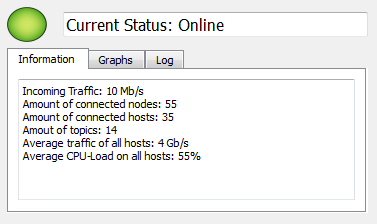
\includegraphics[width=\linewidth]{gui/uebersichtsgui_final_information.png}
	\caption{�bersichtsWidget - Tab Information}
	Hier werden allgemeine Informationen d.h. der Durchschnitt der Auslastung aller Knoten angezeigt, und durch die gr�ne "Ampel" eine korrekte Funktion aller (wichtigen) Knoten signalisiert.
	\end{figure}
	
	\begin{figure}[H]
	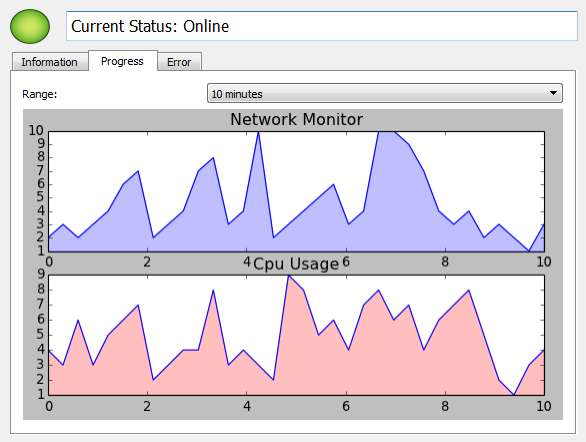
\includegraphics[width=\linewidth]{gui/uebersichtswidget_final_progress.png}
	\caption{�bersichtsWidget - Tab Progress}	
	Die Informationen des InformationsTabs werden hier in Form von Graphen, d.h. im zeitlichen Verlauf dargestellt. Das betrachtete Intervall kann nat�rlich ver�ndert werden.
	\end{figure}
	
	\begin{figure}[H]
	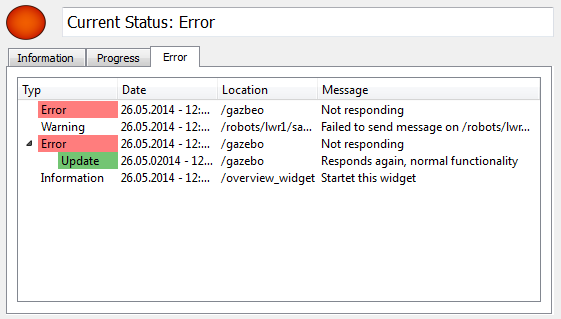
\includegraphics[width=\linewidth]{gui/uebersichtswidget_final_error.png}
	\caption{�bersichtsWidget - Tab Error}
	Im Fehlerfall �ndert sich die Farbe der "Ampel", sodass der Nutzer unmissverst�ndlich erkennt, dass ein Problem existiert, das f�r eine korrekte Funktionsweise behoben werden muss. Im Tab Error findet der Benutzer dann den Log der letzten Fehler um so schnell und einfach herauszufinden, wo das Problem liegt.
	\end{figure}
	
	\newpage

\subsection{Auswahl Widget}
	Dieses Widget zeigt anhand des gerade ausgew�hlten Elements (z.B.durch Anklicken im Nodegraph oder durch Ausw�hlen in einer Liste) detaillierte Information zu dem Element an. Element bedeutet in diesem Fall entweder Knoten oder Host. [TODO: sidn hier topics auch notwendig? glaub nicht...]
	�hnlich wie das �bersichtsWidget ist auch dieses Widget in Tabs organisiert, wobei die Tabs Progress und Error �hnlich funktionieren wie beim �bersichtswidget, weshalb deren Funktionalit�t hier nicht erneut betrachtet werden soll.
\\
	\begin{figure}[H]
	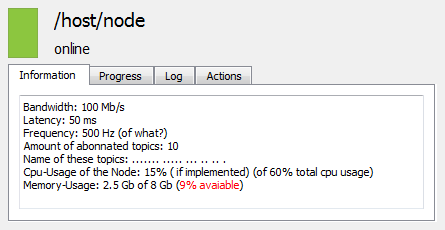
\includegraphics[width=\linewidth]{gui/SelectionWidget_final_info.png}
	\caption{AuswahlWidget - Tab Information}	
	Der Reiter Information bietet wie der Name schon sagt sehr umfangreiche Information �ber das spezifische, gerade ausgew�hlte Element. Diese k�nnen je nach Element (Knoten/Host) unterschiedlich sein, umfassen jedoch u.A. Bandbreite, Latenz, Name der Topics auf denen gesendet wird, Cpu-Auslastung, Speicherauslastung und Andere.
	[TODO: Bild hier noch update, das ("of what?") muss raus]
	\end{figure}
	
	\begin{figure}[H]
	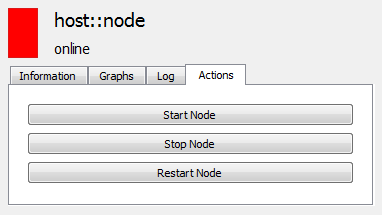
\includegraphics[width=\linewidth]{gui/SelectionWidget_final_actions.png}
	\caption{AuswahlWidget - Tab Actions}	
	Als optionales Feature k�nnen die Knoten im Problemfall neugestartet werden bzw. �berhaupt gestartet werden. Dies erleichtert die Problembehebung erheblich, da diese Funktion aus der Ferne ausgef�hrt werden kann.
	\end{figure}
\newpage






% \end{figure}
	
